% Resumo ISMIR (2 páginas) - TP1 DCC831 IA Generativa para Música, UFMG 2026/2
% Baseado no template oficial ISMIR 2026 (github.com/ismir/paper_templates)
% Compilar: tectonic resumo.tex   (ou pdflatex + bibtex + pdflatex x2)

\documentclass{article}
\usepackage[T1]{fontenc}
\usepackage[utf8]{inputenc}
\usepackage[brazil]{babel}
\usepackage{ismir} % versão final (sem numeração de linhas / anonimização)
\usepackage{amsmath,amssymb,cite,url}
\usepackage{graphicx}
\usepackage{booktabs}
\usepackage{color}

\title{Solos de Guitarra em Contexto por Algoritmo Genético com Fitness Heurística e Licks Idiomáticos}

\oneauthor
  {Thiago Henrique Silva de Almeida}
  {Departamento de Ciência da Computação, Universidade Federal de Minas Gerais\\Matrícula 2024014180 \quad \texttt{thiagohenriquesilva.a@gmail.com}}

% Ajustes ao template: textos em português e sem a nota de licença/atribuição aos
% anais do ISMIR no rodapé da primeira página (este é um trabalho de disciplina).
\makeatletter
\def\abstract{\begin{center}\bf RESUMO\end{center}}
\def\fnum@figure{\textbf{Figura \thefigure}}
\def\fnum@table{\textbf{Tabela \thetable}}
\renewcommand{\permission}{}
\def\thebibliography#1{\section{Referências}\list
  {[\arabic{enumi}]}{\settowidth\labelwidth{[#1]}\leftmargin 1em
  \advance\leftmargin\labelsep\usecounter{enumi}}
  \def\newblock{\hskip .01em plus .01em minus .01em}
  \sloppy\clubpenalty4000\widowpenalty4000\sfcode`\.=1000\relax}
\makeatother

\sloppy

\begin{document}

\maketitle

\begin{abstract}
Este trabalho apresenta um sistema que gera, por algoritmo genético (AG), solos de
guitarra em MIDI (\emph{Musical Instrument Digital Interface}) sobre uma base de
acompanhamento também gerada pelo sistema. A restrição estilística é
a de um solo sobre uma progressão de acordes fixa em um gênero popular; o caso principal
é o blues de 12 compassos na levada \emph{blues shuffle}, e há 19 levadas de 10 gêneros
disponíveis. Cada indivíduo é uma matriz de inteiros sobre uma grade rítmica, avaliada por uma
fitness heurística de 10 critérios de teoria musical e fraseado, calculada em relação
aos acordes e à levada da base. Uma biblioteca de 25 \emph{licks} (frases curtas típicas de
cada estilo) é usada na população inicial e em uma mutação dedicada. Em 5 sementes no
blues, a fitness do melhor indivíduo sobe de 0,80 para $0{,}966\pm0{,}004$ em 300
gerações; sem licks, os critérios de teoria continuam atendidos, mas o solo perde o
vocabulário do gênero.
\end{abstract}

\section{Introdução}\label{sec:introduction}

Improvisar um solo é buscar, sob restrições de harmonia e ritmo, uma frase que soe
dentro do estilo, problema adequado a um AG, que combina variação aleatória com seleção
guiada por uma função de aptidão (fitness). O sistema foi implementado em Python: o usuário escolhe progressão, tonalidade, levada e
andamento em batidas por minuto (bpm); o sistema gera a base (bateria, baixo e harmonia)
e depois evolui um solo avaliado \emph{em contexto}, isto é, contra os acordes e a
levada efetivamente tocados.

\section{Trabalhos Relacionados}

Horner e Goldberg~\cite{horner1991} aplicaram AGs à composição por transformação de
temas. Biles~\cite{biles1994} criou o GenJam, que evolui frases de jazz com fitness
\emph{interativa}, dada por um ouvinte humano; Papadopoulos e
Wiggins~\cite{papadopoulos1998} substituíram o ouvinte por uma fitness automática
baseada em teoria musical, abordagem também seguida aqui. Uma revisão da computação
evolutiva aplicada à música está em~\cite{miranda2007}. Este sistema acrescenta recursos próprios da guitarra (notas duplas e articulações) e
licks protegidos durante a evolução.

\section{Método}

\textbf{Representação.} O solo ocupa $C$ compassos de quatro tempos, e cada tempo é
dividido em $s$ posições (\emph{slots}), num total de $N=4Cs$. O valor de $s$ é a menor
figura rítmica que não ultrapassa 13 notas por segundo no andamento, limite adotado para
manter o solo tocável: no blues shuffle a 100~bpm, cujo \emph{swing} divide o tempo em
três, usa-se a sextina (seis notas por tempo); no thrash metal a 180~bpm, a
semicolcheia (quatro). O indivíduo é uma matriz $G\in\mathbb{Z}^{4\times N}$. A linha de melodia
guarda, em cada posição, uma pausa ($-1$), a sustentação da nota anterior ($-2$) ou o
ataque de uma nota, representada pelo índice $0..P{-}1$ na escala do solo, limitada à
extensão de Sol 3 a Ré 6 ($P$ entre 17 e 24 notas). As outras linhas guardam a nota
dupla (uma segunda nota tocada junto, em semitons de distância), a articulação
(\emph{bend}, em que a corda é puxada para subir a nota, ou deixar a nota soar) e a
origem (qual lick escreveu aquela posição, informação que não altera o som). A escala
do solo vem da levada e do modo da música (ex.: modo frígio, escala menor com a segunda
abaixada, no thrash metal) ou é escolhida pelo usuário entre 14 opções.

\textbf{População inicial.} Foram usados 120 indivíduos, construídos tempo a tempo:
cada tempo recebe uma pausa, a sustentação da nota anterior, de uma a três notas ou uma
sequência rápida de notas. As alturas seguem um passeio aleatório pela escala, que gera
melodias com passos curtos, e cada compasso recebe um lick com probabilidade 0,3. Os
licks são sorteados conforme a afinidade com o gênero e ajustados ao acorde e à escala.

\textbf{Fitness.} A fitness é a média ponderada $F=\sum_c w_c\,s_c/\sum_c w_c$ dos
critérios $s_c\in[0,1]$ da Tabela~\ref{tab:fitness}. Os alvos de densidade (notas por
tempo) e de \emph{shred} (fração das notas em sequências rápidas e virtuosísticas)
dependem do gênero. A harmonia recebeu o maior peso por ser o critério que mais afeta a sensação de
``nota errada''.

\begin{table}[t]
\centering\footnotesize
\begin{tabular}{@{}l l r@{}}
\toprule
Critério & O que mede & $w_c$ \\
\midrule
harmonia & notas do acorde nos tempos e nas notas longas & 3,0\\
consonância & pouco tempo em notas que colidem com o acorde & 2,0\\
intervalos & predomínio de passos curtos na escala & 2,0\\
densidade & notas por tempo próximas do alvo & 1,5\\
\emph{shred} & fração de notas rápidas próxima do alvo & 1,5\\
coerência & ataques em figuras rítmicas regulares & 1,5\\
fraseado & 12\% de pausa, sem notas picotadas & 1,5\\
motivo & ritmo parecido entre compassos vizinhos & 1,5\\
final & nota longa na tônica no último compasso & 1,5\\
idioma & parte do solo coberta por licks do gênero & 1,5\\
\bottomrule
\end{tabular}
\caption{Critérios da fitness heurística e pesos padrão.}
\label{tab:fitness}
\end{table}

\textbf{Seleção, cruzamento e mutação.} Os pais foram escolhidos por torneio de tamanho
3: sorteiam-se três indivíduos e o de maior fitness é selecionado, o que mantém uma
pressão seletiva moderada. Foi utilizado elitismo de 2 indivíduos, copiados sem
alteração para a geração seguinte para que o melhor solo encontrado nunca se perca. O
cruzamento, aplicado com probabilidade 0,9, é de dois pontos, e os cortes só ocorrem
entre compassos para não partir uma nota ou frase ao meio. Cada filho passa por até
quatro tentativas de mutação, cada uma com probabilidade 0,3; os dez tipos incluem
mover uma nota na escala, copiar um compasso transposto (o que cria motivos), inserir
uma sequência rápida, mudar a nota dupla ou a articulação e inserir um lick. Mutações que alteram um lick são
desfeitas com probabilidade 0,7, para que os licks variem devagar.

\textbf{Parada e síntese.} A evolução termina após 300 gerações ou 80 sem melhora do
melhor indivíduo; assim, cada execução leva menos de um minuto.
O áudio, só para audição, é sintetizado com o FluidSynth.

\section{Resultados}

\begin{figure}[t]
\centerline{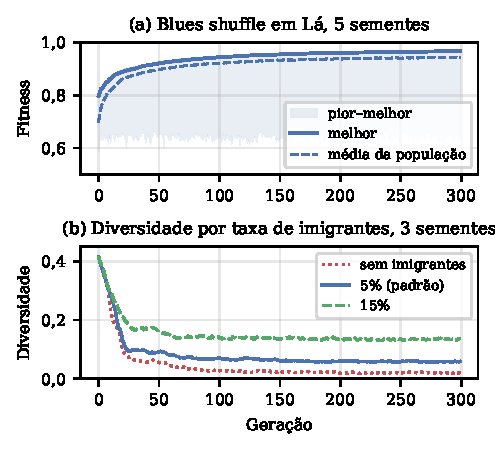
\includegraphics[width=\columnwidth]{fitness.pdf}}
\caption{Evolução da fitness. (a) Melhor indivíduo (média $\pm$ desvio-padrão), média
da população e faixa entre o pior e o melhor; 5 sementes, parâmetros padrão. (b) Melhor
indivíduo ao variar um hiperparâmetro por vez.}
\label{fig:fitness}
\end{figure}

\begin{table}[t]
\centering\footnotesize\setlength{\tabcolsep}{4pt}
\begin{tabular}{@{}l c c c@{}}
\toprule
Configuração & $F$ final & Ger.\ até 0,95 & Licks \\
\midrule
blues shuffle, padrão (5 sem.) & $0{,}966\pm0{,}004$ & 133 & 11,4\\
\quad mutação 0,1 & $0{,}964\pm0{,}003$ & 161 & 10,7\\
\quad mutação 0,6 & $0{,}960\pm0{,}002$ & 159 & 12,0\\
\quad inicialização uniforme & $0{,}964\pm0{,}004$ & 129 & 13,0\\
\quad sem licks & $0{,}878\pm0{,}006$ & -- & 0\\
\midrule
thrash metal (Mi menor) & $0{,}936\pm0{,}003$ & -- & 7,7\\
hard rock (Mi menor) & $0{,}950\pm0{,}004$ & 176$^*$ & 9,7\\
funk (Mi menor) & $0{,}973\pm0{,}004$ & 58 & 10,0\\
balada pop (Dó maior) & $0{,}958\pm0{,}006$ & 175 & 10,0\\
\bottomrule
\end{tabular}
\caption{Fitness final, geração em que o melhor indivíduo atinge 0,95 (média entre
sementes) e número de licks com pelo menos metade das notas intactas no solo final.
Blues shuffle: 12 compassos em Lá a 100~bpm, tocados duas vezes. Três sementes por
linha, salvo indicação. $^*$Só uma das três sementes atingiu 0,95.}
\label{tab:results}
\end{table}

\textbf{Protocolo.} Foram variados, um de cada vez, a semente, a taxa de mutação, a
inicialização, a presença de licks e o gênero, em 29 execuções
(Tabela~\ref{tab:results}), todas reproduzíveis por um script incluído no repositório.

\textbf{Convergência.} A Figura~\ref{fig:fitness}a mostra o comportamento típico: subida
rápida nas primeiras 50 gerações (de 0,80 para 0,92) e, depois, ganhos pequenos até a
geração 300 (0,94 na geração 100 e 0,96 na 200). A média da população acompanha o
melhor de perto, sinal de perda de diversidade cedo. Sementes diferentes dão solos diferentes com fitness quase igual.

\textbf{Hiperparâmetros.} Com mutação 0,3, o melhor indivíduo chegou a 0,95 cerca
de 27 gerações antes do que com 0,1 (pouca exploração) ou 0,6 (desfaz frases boas),
mas as fitness finais ficam a um desvio-padrão umas das outras. A inicialização por
passeio aleatório começa acima da uniforme (0,80 contra 0,78), vantagem que some. Sem licks, o
critério de idioma fica em zero e limita $F$ a $15{,}5/17\approx0{,}912$; descontado
isso, os demais critérios ficam tão altos quanto no padrão (0,963). Ou seja, a
teoria é atendida sem o vocabulário do gênero, que vem só dos licks.

\textbf{Gêneros.} O funk converge mais rápido (58 gerações), possivelmente porque a progressão alterna
só dois acordes e as frases sincopadas dos licks se encaixam nela. O thrash metal é o
caso mais difícil: os \emph{power chords}, acordes formados só pela fundamental e pela
quinta, oferecem apenas duas notas do acorde, o que reduz a harmonia para 0,84. No hard rock, a densidade fica abaixo do alvo (0,83).

% TODO(autor): conferir a descrição qualitativa abaixo ouvindo os MP3.
\textbf{Músicas.} A pasta \texttt{musicas/} do
repositório\footnote{\url{https://github.com/ThiagoHSAl/guitar-solo-ga}} traz cinco
peças (MP3 e MIDI) com gênero, escala, andamento e semente diferentes: blues shuffle em Lá (escala blues, 100~bpm), thrash metal em Mi (modo
frígio, 180~bpm), hard rock em Mi (modo dórico, escala menor com a sexta elevada,
126~bpm), funk em Mi (dórico, 96~bpm) e balada pop em Dó (escala maior, 72~bpm).
Os solos usam notas do acorde nos tempos fortes, alternam trechos rápidos e notas
longas com bends e terminam na tônica.

\section{Discussão e Trabalhos Futuros}

A principal limitação é que a fitness mede conformidade com regras, não qualidade
musical: valores acima de 0,95 são atingidos com facilidade, e diferenças pequenas de
$F$ não correspondem necessariamente a diferenças audíveis. Pesos, alvos e licks foram definidos à mão, o que introduz um viés do autor, e não
houve avaliação com ouvintes. Como extensões, são
propostos: (i) um teste de audição; (ii) uma fitness interativa ou híbrida, como no
GenJam~\cite{biles1994}; (iii) aprender alvos e licks de um corpus de solos transcritos;
e (iv) otimização multiobjetivo, como o NSGA-II (\emph{Non-dominated Sorting Genetic
Algorithm II}), em vez de pesos fixos.

\bibliography{refs}

\end{document}
